% TikZ code representing the transformation of a graph to a d-regular instance
% where each vertex of degree d_v is replaced by a cluster of d_v vertices.
% The nodes inside each cluster are arranged as regular polygons, oriented
% to face directly towards the edges connected to them.
% Generated by Antigravity on 2026-07-19.

% Parameter describing how large around the nodes the cloud should be
\providecommand{\cloudsize}{0.65}

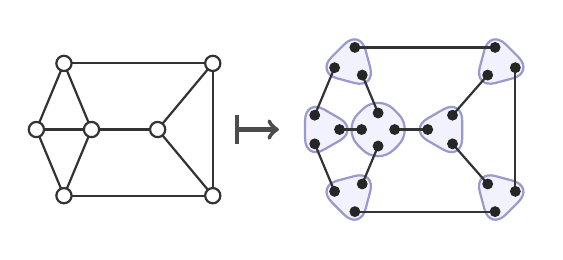
\begin{tikzpicture}[
    scale=0.7,
    vertex/.style={circle, draw=black!80, fill=white, minimum size=5.5pt, inner sep=0pt, thick},
    mini/.style={circle, draw=black!85, fill=black!85, minimum size=3.5pt, inner sep=0pt},
    edge/.style={thick, draw=black!80},
    blob/.style={draw=blue!50!black!40, fill=blue!5, thick, rounded corners=8pt}
]

    % ==================== LEFT GRAPH ====================
    % Edges (drawn first so nodes sit on top)
    \draw[edge] (-1.6, 0) -- (-1.1, 1.2);
    \draw[edge] (-1.6, 0) -- (-1.1, -1.2);
    \draw[edge] (-1.6, 0) -- (-0.6, 0);
    \draw[edge] (-0.6, 0) -- (-1.1, 1.2);
    \draw[edge] (-0.6, 0) -- (-1.1, -1.2);
    \draw[edge] (-0.6, 0) -- (0.6, 0);
    \draw[edge] (-1.1, 1.2) -- (1.6, 1.2);
    \draw[edge] (-1.1, -1.2) -- (1.6, -1.2);
    \draw[edge] (0.6, 0) -- (1.6, 1.2);
    \draw[edge] (0.6, 0) -- (1.6, -1.2);
    \draw[edge] (1.6, 1.2) -- (1.6, -1.2);

    % Vertices
    \node[vertex] at (-1.6, 0) {};
    \node[vertex] at (-1.1, 1.2) {};
    \node[vertex] at (-1.1, -1.2) {};
    \node[vertex] at (-0.6, 0) {};
    \node[vertex] at (0.6, 0) {};
    \node[vertex] at (1.6, 1.2) {};
    \node[vertex] at (1.6, -1.2) {};


    % ==================== MAPPING ARROW ====================
    \draw[|->, ultra thick, draw=black!70] (2.0, 0) -- (2.8, 0);


    % ==================== RIGHT GRAPH ====================
    % Blobs / Clusters (Regular rounded polygons in the background, scaled by \cloudsize)
    \draw[blob] ({3.6 + \cloudsize*cos(0)}, {\cloudsize*sin(0)}) -- ({3.6 + \cloudsize*cos(120)}, {\cloudsize*sin(120)}) -- ({3.6 + \cloudsize*cos(240)}, {\cloudsize*sin(240)}) -- cycle;
    \draw[blob] ({4.1 + \cloudsize*cos(315)}, {1.2 + \cloudsize*sin(315)}) -- ({4.1 + \cloudsize*cos(75)}, {1.2 + \cloudsize*sin(75)}) -- ({4.1 + \cloudsize*cos(195)}, {1.2 + \cloudsize*sin(195)}) -- cycle;
    \draw[blob] ({4.1 + \cloudsize*cos(45)}, {-1.2 + \cloudsize*sin(45)}) -- ({4.1 + \cloudsize*cos(165)}, {-1.2 + \cloudsize*sin(165)}) -- ({4.1 + \cloudsize*cos(285)}, {-1.2 + \cloudsize*sin(285)}) -- cycle;
    \draw[blob] ({4.6 + \cloudsize*cos(0)}, {\cloudsize*sin(0)}) -- ({4.6 + \cloudsize*cos(90)}, {\cloudsize*sin(90)}) -- ({4.6 + \cloudsize*cos(180)}, {\cloudsize*sin(180)}) -- ({4.6 + \cloudsize*cos(270)}, {\cloudsize*sin(270)}) -- cycle;
    \draw[blob] ({5.8 + \cloudsize*cos(180)}, {\cloudsize*sin(180)}) -- ({5.8 + \cloudsize*cos(300)}, {\cloudsize*sin(300)}) -- ({5.8 + \cloudsize*cos(60)}, {\cloudsize*sin(60)}) -- cycle;
    \draw[blob] ({6.8 + \cloudsize*cos(225)}, {1.2 + \cloudsize*sin(225)}) -- ({6.8 + \cloudsize*cos(345)}, {1.2 + \cloudsize*sin(345)}) -- ({6.8 + \cloudsize*cos(105)}, {1.2 + \cloudsize*sin(105)}) -- cycle;
    \draw[blob] ({6.8 + \cloudsize*cos(135)}, {-1.2 + \cloudsize*sin(135)}) -- ({6.8 + \cloudsize*cos(255)}, {-1.2 + \cloudsize*sin(255)}) -- ({6.8 + \cloudsize*cos(15)}, {-1.2 + \cloudsize*sin(15)}) -- cycle;

    % Inter-cluster Edges
    \draw[edge] (3.45, 0.26) -- (3.81, 1.122);        % A'_B to B'_A
    \draw[edge] (3.45, -0.26) -- (3.81, -1.122);      % A'_C to C'_A
    \draw[edge] (3.9, 0) -- (4.3, 0);                  % A'_D to D'_A
    \draw[edge] (4.312, 0.988) -- (4.6, 0.3);          % B'_D to D'_B
    \draw[edge] (4.312, -0.988) -- (4.6, -0.3);        % C'_D to D'_C
    \draw[edge] (4.178, 1.49) -- (6.722, 1.49);        % B'_F to F'_B
    \draw[edge] (4.178, -1.49) -- (6.722, -1.49);      % C'_G to G'_C
    \draw[edge] (4.9, 0) -- (5.5, 0);                  % D'_E to E'_D
    \draw[edge] (5.95, 0.26) -- (6.588, 0.988);        % E'_F to F'_E
    \draw[edge] (5.95, -0.26) -- (6.588, -0.988);      % E'_G to G'_E
    \draw[edge] (7.09, 1.122) -- (7.09, -1.122);      % F'_G to G'_F

    % Mini-vertices (Oriented Regular Polygons)
    % Cluster A' (Triangle pointing right / flipped to face neighbor D')
    \node[mini] at (3.9, 0) {};
    \node[mini] at (3.45, 0.26) {};
    \node[mini] at (3.45, -0.26) {};

    % Cluster B' (Triangle pointing down-right / rotated to face edges)
    \node[mini] at (4.312, 0.988) {};
    \node[mini] at (4.178, 1.49) {};
    \node[mini] at (3.81, 1.122) {};

    % Cluster C' (Triangle pointing up-right / rotated to face edges)
    \node[mini] at (4.312, -0.988) {};
    \node[mini] at (3.81, -1.122) {};
    \node[mini] at (4.178, -1.49) {};

    % Cluster D' (Square/Diamond)
    \node[mini] at (4.9, 0) {};
    \node[mini] at (4.6, 0.3) {};
    \node[mini] at (4.3, 0) {};
    \node[mini] at (4.6, -0.3) {};

    % Cluster E' (Triangle pointing left)
    \node[mini] at (5.5, 0) {};
    \node[mini] at (5.95, 0.26) {};
    \node[mini] at (5.95, -0.26) {};

    % Cluster F' (Triangle pointing down-left / rotated to face edges)
    \node[mini] at (6.588, 0.988) {};
    \node[mini] at (7.09, 1.122) {};
    \node[mini] at (6.722, 1.49) {};

    % Cluster G' (Triangle pointing up-left / rotated to face edges)
    \node[mini] at (6.588, -0.988) {};
    \node[mini] at (7.09, -1.122) {};
    \node[mini] at (6.722, -1.49) {};

\end{tikzpicture}
